\documentclass{article}
\usepackage[utf8]{inputenc}

\title{Laboratorio03_INTELIGENCIA_NEGOCIOS}
\author{edwartbalcon}
\date{Septiembre 2021}

\usepackage[utf8]{inputenc}
\usepackage[spanish]{babel}
\usepackage{natbib}
\usepackage{graphicx}

\begin{document}

\title{Caratula}

\begin{titlepage}
\begin{center}
\begin{Large}
\textbf{UNIVERSIDAD PRIVADA DE TACNA} \\
\end{Large}
\vspace*{-0.025in}
\begin{figure}[htb]
\begin{center}

\includegraphics[width=6cm]{./images/logo_UPT}
\end{center}
\end{figure}
\vspace*{-0.025in}
\begin{Large}
\textbf{FACULTAD DE INGENIERIA} \\
\end{Large}
\vspace*{0.05in}
\begin{Large}
\textbf{Escuela Profesional de Ingeniería de Sistema} \\
\end{Large}


\vspace*{0.4in}

\vspace*{0.1in}
\begin{Large}
\textbf{Informe de laboratorio 07: Kinesis Data Streams} \\
\end{Large}

\vspace*{0.3in}
\begin{Large}
\textbf{Curso: Inteligencia de negocios} \\
\end{Large}

\vspace*{0.3in}
\begin{Large}
\textbf{DOCENTE: Ing. Patrick Cuadros Quiroga} \\
\end{Large}

\vspace*{0.2in}
\vspace*{0.1in}
\begin{large}

\begin{Large}
\textbf{Alumno: Balcon Coahila, Edwart Juan\hfill	(2013046516) } \\
\end{Large}

\vspace*{0.15in}
\begin{Large}
\textbf{Tacna – Perú} \\
\end{Large}

\vspace*{0.05in}
\begin{Large}
\textbf{2021 } \\
\end{Large}

\end{large}
\end{center}

\end{titlepage}


\newpage

\section{ Realizar los siguientes pasos para el laboratorio }

\textbf{1.1.  Entrar a la consola de AWS.}

    
\textbf{1.2.  Ir al servicio de Kinesis Data Streams, clic en Crear secuencia de datos}

\begin{center}
		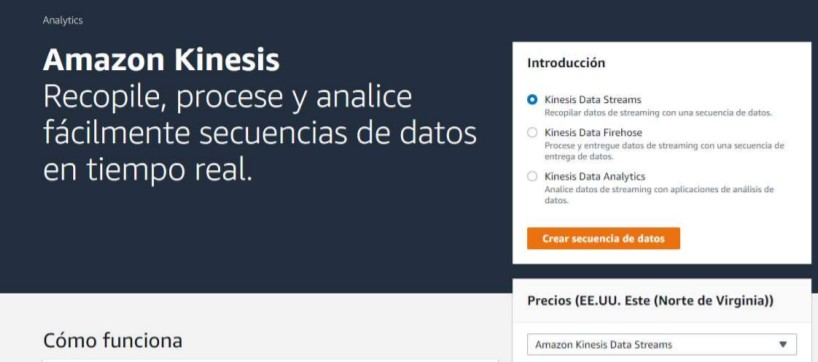
\includegraphics[width=15cm]{./images/1} 
	\end{center}
	
\textbf{1.3.  Crear el stream con el nombre de streamVuelos, y luego siguiente y otra vez siguiente.
En el campo Number of fragmentos ingresamos 1 y clic en Crear secuencia de datos.
}

    \begin{center}
		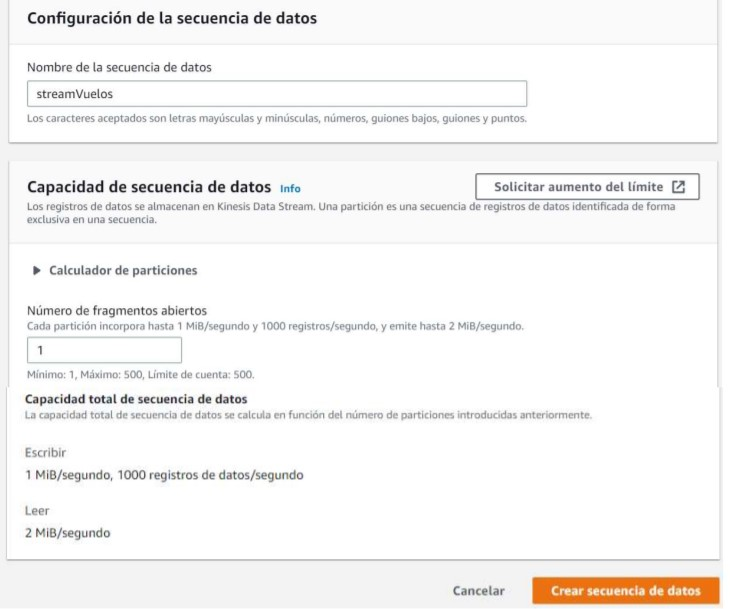
\includegraphics[width=15cm]{./images/2} 
	\end{center}

\newpage
\textbf{1.4.   El stream se ha creado
}

    \begin{center}
		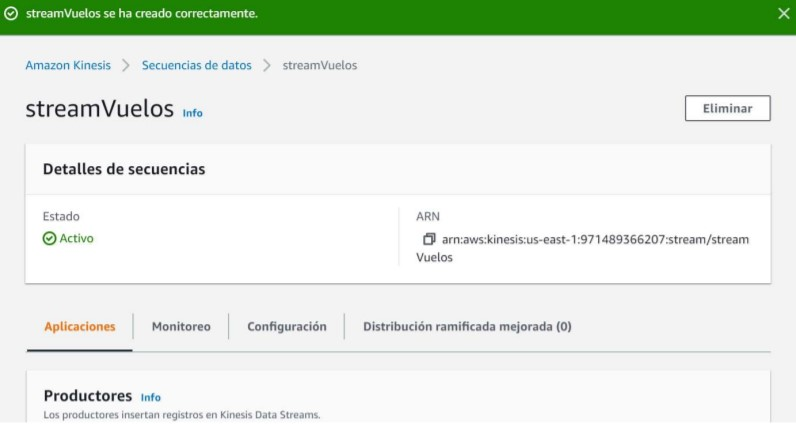
\includegraphics[width=15cm]{./images/3} 
	\end{center}
	
	\newpage
\textbf{1.5.   Entramos a la EC2 que hemos creado
Ejecutar los siguientes comandos en el terminal del linux:
}

    \begin{center}
		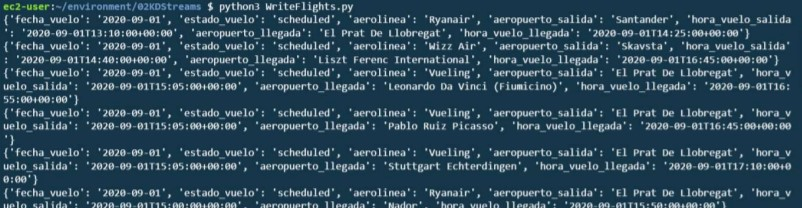
\includegraphics[width=15cm]{./images/4} 
	\end{center}
	
	\newpage
    \begin{center}
		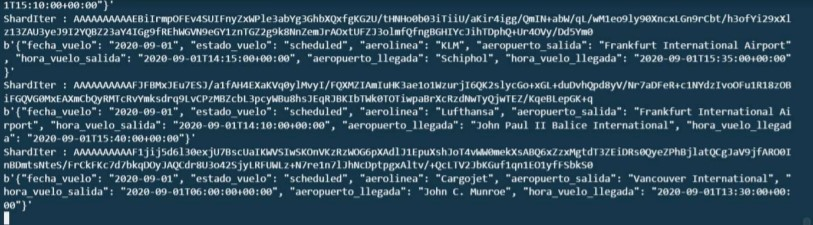
\includegraphics[width=15cm]{./images/5} 
	\end{center}

\end{document}